\documentclass[../main.tex]{subfiles}
\begin{document}

\chapter{Lecture 18 - 12-05-2020}

\section{Kernel functions}

We use a notion of \red{feature expansion}. They are different but somehow they reach something similar. In fact Linear classifier have high bias.
\\
Linear predictor use hyper plane as basic brick to build prediction.

\subsection{Feature expansion}
Given $\phi : \barra{R}^d \longrightarrow V \qquad V$ is typically $\barra{R}^N$ \quad $N >> d$
\\\\
For example:\\
$d = 2 \quad N = 6 \quad \phi = \barra{R}^2 \longrightarrow \barra{R}^6 \quad$ $$\phi(x_1,x_2) = (1,x_1^2,x_2^2,x_1,x_2,x_1 x_2)$$
We have a homogenous hyper plane.
\\
$w \in \barra{R}^6 \ \{ z \in \barra{R}^6 : w^T z = 0 \} \qquad z = \phi(x) \qquad x \in \barra{R}^2$
\\
$$
\forall x \in \barra{R}^2 \qquad w^t \phi(x) = w_1+w_2 x_1^2 + w_3 x_2^2 + w_4 x_1 + w_5 x^2 + w_6 x_1 x_2 = 0
$$\
$$
w^T \phi(x) = 0 
$$\\
\begin{figure}[h]
    \centering
    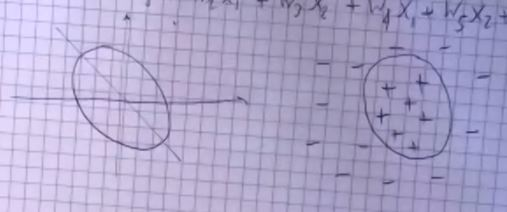
\includegraphics[width=0.6\linewidth]{../img/lez18-img1.JPG}
    \caption{} 
    %\label{fig:}
\end{figure}\\
$$
\phi : \barra{R}^d \longrightarrow \barra{R}^N \qquad \Pi_{s=1}^{M} x_{Vs} \quad v \in \{1,...d\}^k \quad k = 0, ..., n 
$$
$$
h(x) = sgn (w^T \phi(x)) \qquad w^T \phi(x) = \sum_{i= 1}^{N} w_i \phi(x)_i
$$
The problem of this feature expansion is the degree of the monomials!
\\
$$
N = \sum_{i = 0}^{n} | \{ 1,...d \}^k | = \sum_{k = 0}^{n} d^k  = \frac{d^{n+1}-1}{d-1} = \Theta (d^n)
$$
So it's exponential! But this feature expansion can be implemented in a efficient way.
\subsection{Kernels implements feature expansion (Efficiently}

$ w^T \phi(x) $ \quad Perception $ w \leftrightarrow w + y_t x_t I \{y_t w^T x_t \leq 0 \} $ MANCA quadlcosa
\\
$$
w = \sum_{s\in S} y_s x_s \leadsto \sum_{s \in S} y_s \phi (x_s) 
$$ 
where $S$ is a subset of traning set where updates occurred.
\\
Every time i make a mistake i add some of this product of data points. \\
If I run this using example that are images accourding to some feature expansion map $(\phi)$, I will get the perceptron after the mapping.
$$
w^T \phi(x) = \sum_{s \in S} y_s \phi(x)^T \phi(x_s)
$$
It's a inner problem and can have exponentially degree of the component.
\\
\red{Kernels help me compute this inner product $ \phi(x)^T \phi(x_s) $ quickly}
\\
$$
\phi: \barra{R}^2 \longrightarrow \barra{R}^6 \qquad \phi(x_1,x_2) = (1, \ x_1^2, \ x_2^2, \ \sqrt[]{2} x_1, \ \sqrt[]{2} x_2, \ \sqrt[]{2} x_1 x_2)
$$

$$
\phi(x)^T \phi(z) \ = \ 1+x_1^2 z_1^2 + x_2^2 z_2^2 + 2 x_2 z_2 + 2 x_1 x_2 z_1 z_2 \ = \ (1+x^T z ) ^2 \ = \ k(x,z)
$$\
$$
w^T\phi(x) = \sum_{s \in S} y_s \ k(x,x_2)
$$
\\
$k(x,z)$ implements $\phi(x)^T \phi(z)$ \quad $\forall x, z $ and $\phi$ defined as before
\\\\
How to we generalise this?
$$
k_n \left(x, x' \right) = (1+x^2 x' ) ^n
$$
This is called polynomial kernel.
\\\\
I want to check now what is the $\phi$ for $K_n$?
\\
I want to compute $\phi$ s.t. $\phi(x)^T \phi(x') = k_n(x,x') = (1+x^T x' ) ^n$
\\
We can use Newtons bynomial theorem:
\\
$$(1+x^T x')^n = \sum_{k=0}^n \binom{n}{k} (x^t x')^k $$
$$
(x^T x')^k = \left( \sum_{i=1}^{d} x_i x'_i \right)^k = \sum_{v \in \{ 1,...d \}^k} \left( \prod_{s=1}^{k} x_{Vs} x'_{Vs} \right)
$$
$$
\phi(x) = \left( \sqrt[]{\binom{n}{k}} \prod_{s=1}^{k} x_{Vs} \right) \qquad k = 0,..., n \qquad v \in \{1,...d\}^k
$$
When I am using polynomial kernel I am implicitely using the feature expansion ...
\\
Can an algorithm work using kernel?
\\
Perceptron works!
\\\\
$
S = 0 \\
For \ t = 1,2,... \\
1)$ Get $(x_t,y_t)\\
2) \  \hat{y}_t = sgn\left( \sum_{s \in S} y_s \ K(x ,x_s \right)
\\
3)
$
If $ \hat{y}_t \neq y_t \quad S \longleftarrow S \cup \{t\} \qquad w \leftarrow w + y_t \phi(x_t) $
\\\\
$$
\textit{So I am representing y as a sum and not as a vector. In fact, \ }  w = \sum_{s \in S} y_s \phi(x_s)$$ù

\section{Gaussian Kernel}

$$\gamma > 0 \qquad k_{\gamma} (x, x') = \exp \left( - \frac{1}{2 \ \gamma} \ \| x- x' \|^2 \right)
$$
$$
e^{- \frac{1}{2 \ \gamma} \ \left(x - x' \right) ^2}
$$
I can controll the distribution changing the value of $\gamma$
\begin{figure}[h]
    \centering
    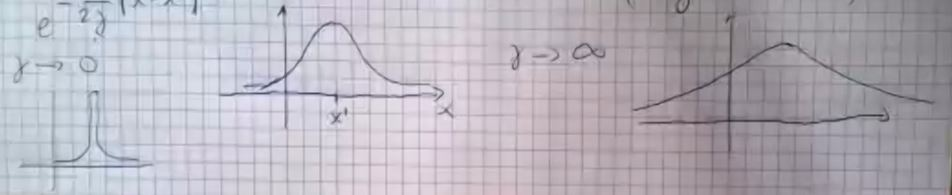
\includegraphics[width=0.8\linewidth]{../img/lez18-img2.JPG}
    \caption{} 
    %\label{fig:}
\end{figure}\\\\\\
$$
\hat{y}_t = sgn \left( \sum_{s \in S} y_s \ K_{\gamma} (x, x_s) \right)
$$
\begin{figure}[h]
    \centering
    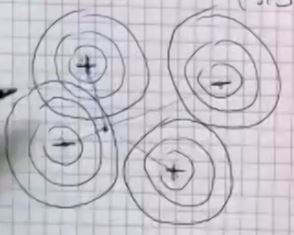
\includegraphics[width=0.6\linewidth]{../img/lez18-img3.JPG}
    \caption{} 
    %\label{fig:}
\end{figure}\\
Negative or positive gaussin component looking at the distance. 
\\
Now I want to compute: $ \phi_\gamma : \barra{R}^n \longrightarrow V$
\\\\
$$
\exp \left( - \frac{1}{2 \ \gamma} \| x- x'\|^2 \right) = \exp \left(  - \frac{1}{2 \ \gamma} \left( \| x \|^2 + \| x'\|^2 \right) \right) \cdot \exp \left( \frac{1}{\gamma} x^T x'\right) =
$$
where $e = x+ \frac{x^2}{!2} ... $
$$
= \exp \left(  - \frac{1}{2 \ \gamma} \| x \|^2 \right) \cdot \exp \left(  - \frac{1}{2 \ \gamma} \| x' \|^2 \right) \cdot \sum_{n=0}^{\infty} \frac{1}{n! } \frac{\left( x^T x' \right)^2}{\gamma^n}
$$
Gaussian Kernel is a linear combination of infinitely many poly kernels.
\\
The higher I go the small is $n!$. Gaussian kernel mapping into  a space that is very large. So large that it has infinitely many dimension. Why? Because each polynomial kernel  maps to infinitely dimensions.
\\\\
$\phi_\gamma$ maps $\barra{R}^d$ into a space of infinitely many dimensions.
\\
$$\phi_\gamma : \barra{R}^d \rightarrow V \qquad
k_\gamma \left(x, x'\right) = \phi_\gamma(x)^T \phi_\gamma(x)
$$
It maps to infinetely many dimension, so it maps to a function!
\\
\bred{$
\phi_\gamma(x)
$ is a function.}
\\
In general, when I learn a linear predictor using $k_\gamma$ 
\\ I learn $\sum_s \alpha_s \ k(x_s,\cdot) = f$
\\
$
w^T \phi(x)
$
$$
H_\gamma \equiv \{  \ \sum_{i = 1}^{N} \alpha_i \ k \left(x_i, \bred{$\cdot$} \right) \ : \ x_1,...,x_N \in \barra{R}^d, \ \alpha_1,..., \alpha_N \in \barra{R}, \ N \in \barra{N} \ \}
$$
\bred{Theorem}\\
$ \forall \gamma > 0 \ \forall f : \barra{R}^d \rightarrow \barra{R} $ continous, $\forall \varepsilon > 0 $
\\
$
\exists g \in H_\gamma 
$ that approximates $f$ with error $\varepsilon$
\\
We define a function with H. We see the \bred{$\cdot$} and this tell us is a function. So we can evaluate every kind of $x$ point in \bred{$\cdot$} position.
\\\\
We are able to get a super parametric algorithm and transform it in a non-parametric algorithm. Parametric algorithms is defined by an arbitrary number of parameter we cannot adapt it for every case.
\\\\
Gaussian Kernels enable consistency by using feature expansion with infinitely many components.
\end{document}